\documentclass[serif,mathserif,final]{beamer}
\mode<presentation>{\usetheme{Lankton}}
\usepackage{mathtools,amsmath,amsfonts,amssymb,pxfonts,xspace,bm}
\usepackage{graphicx,caption,courier}
\graphicspath{{../figures/}}
%\usepackage[orientation=landscape,size=custom,width=70,height=40,scale=.6,debug]{beamerposter}
%\usepackage[orientation=landscape,size=custom,width=101,height=65,scale=1,debug]{beamerposter}
%\usepackage[orientation=portrait, size=a0,scale=1.2]{beamerposter}
\usepackage[orientation=portrait,size=custom,width=80,height=92,scale=1.15,debug]{beamerposter}
%\usepackage[orientation=landscape,size=custom,width=47,height=37,scale=.4,debug]{beamerposter}
\usepackage{booktabs} % for tabular toprule, bottomrule, midrule. Better than hline.

%-- Header and footer information ----------------------------------
\newcommand{\footleft}{\bfseries{http://dahl.byu.edu}}
\newcommand{\footright}{\bfseries{warr@stat.byu.edu}}
\title{Attraction Indian Buffet Distribution}
\author{David Dahl \& Richard Warr}
\institute{Brigham Young University}
%-------------------------------------------------------------------

%-- My Functions----------------------------------------------------
\def\prodl#1#2#3{\prod\limits_{#1=#2}^{#3}}
\def\suml#1#2#3{\sum\limits_{#1=#2}^{#3}}
\def\sums#1#2#3{\sum\limits_{#1:#2}^{#3}}
\def\ds{\displaystyle}
\def\hik{\ds\frac{\suml{j}{1}{i-1}\lambda(\sigma_j,\sigma_i)~z_{j,k}}
        {\suml{j}{1}{i-1}\lambda(\sigma_j,\sigma_i)}}
%\def\hik{ \suml{j}{1}{i-1}\lambda(\sigma_j,\sigma_i)~z_{j,k} ~\bigg/
%          \suml{k}{1}{y_i}\suml{j}{1}{i-1}\lambda(\sigma_j,\sigma_i)~z_{j,k}}
\def\lb{\left \{ }
\def\rb{\right \}}

%-------------------------------------------------------------------
%-- Main Document --------------------------------------------------
\begin{document}
\begin{frame}{}
  \vskip-1cm



  \begin{columns}[t]




    %-- Column 1 ---------------------------------------------------
    \begin{column}{0.4\linewidth}

      %-- Block 1-1
      
\begin{block}{Abstract}
        We propose the attraction Indian buffet distribution (aIBD) as 
        a latent feature model indexed by pairwise distances.
        Items that are ``close'' are more likely to share features.
        %an alternative to the ddIBP. 
        The aIBD extends the Indian buffet process (IBP) in the same way
        that the Ewens-Pitman attraction (EPA) distribution extends the
        Chinese restuarant process (CRP).
        %The aIBD makes use of similarity, which Dahl et al. (2014) use in the
        %Ewen-Pitman attraction (EPA) distribution. 
        We draw comparisons between the aIBD and the distance dependent Indian
        buffet process (ddIBP). We show that the aIBD maintains the expected
        number of columns of the IBP, has an explicit probability mass
        function, and reduces to the IBP in special cases.

        %Implementations of the IBP to include distance information have been
        %studied and introduced by researchers such as Gershman et al. (2012).
        %The distance-dependent Indian buffet process (ddIBP) is one such
        %implementation. It reduces to the regular IBP under certain conditions,
        %and preserves many of the properties of the IBP. We propose the
        %Attraction Indian Buffet process (aIBD) as an alternative to the ddIBP.
        %The aIBD makes use of attraction information that Dahl et al. (2014)
        %use in the Ewen-Pitman attraction (EPA) distribution. We will draw
        %comparisons between the aIBD and the ddIBP. We also show that the aIBD
        %preserves the dimensions of the IBP, has an explicit p.m.f., and
        %reduces to the IBP when all items are equidistant.
      \end{block}

\vspace{1em}

           \begin{block}{Properties of IBP Maintained}
        \vspace{.5em}
        \begin{center}
          \begin{tabular}{lrr}
            \toprule
            \textbf{Property} & \textbf{aIBD} & \textbf{ddIBP} \\ \midrule
            Explicit pmf & {\color{red}Yes} & {\color{red}No} \\
            Expected non-zero columns equal to that of IBP & {\color{red}Yes} & {\color{red}No} \\
              Expected row sums equal to that of IBP & Yes & Yes \\
              Expected column sums equal to that of IBP & No & No \\
            \bottomrule
          \end{tabular}
          %\vspace{.5em}
          %\captionof{table} {Comparison of the ddIBP and our aIBD, showing which 
          %                   properties of the IBP are presrved.}
        \end{center}
      \end{block}

\vspace{1em}

\begin{block}{Temperature Plots}
        \begin{figure}[htb]
          \centering
          %\includegraphics[width=.99\columnwidth]{temperature}
          \href{http://luiarthur.github.io/posts/ibp/may/26}{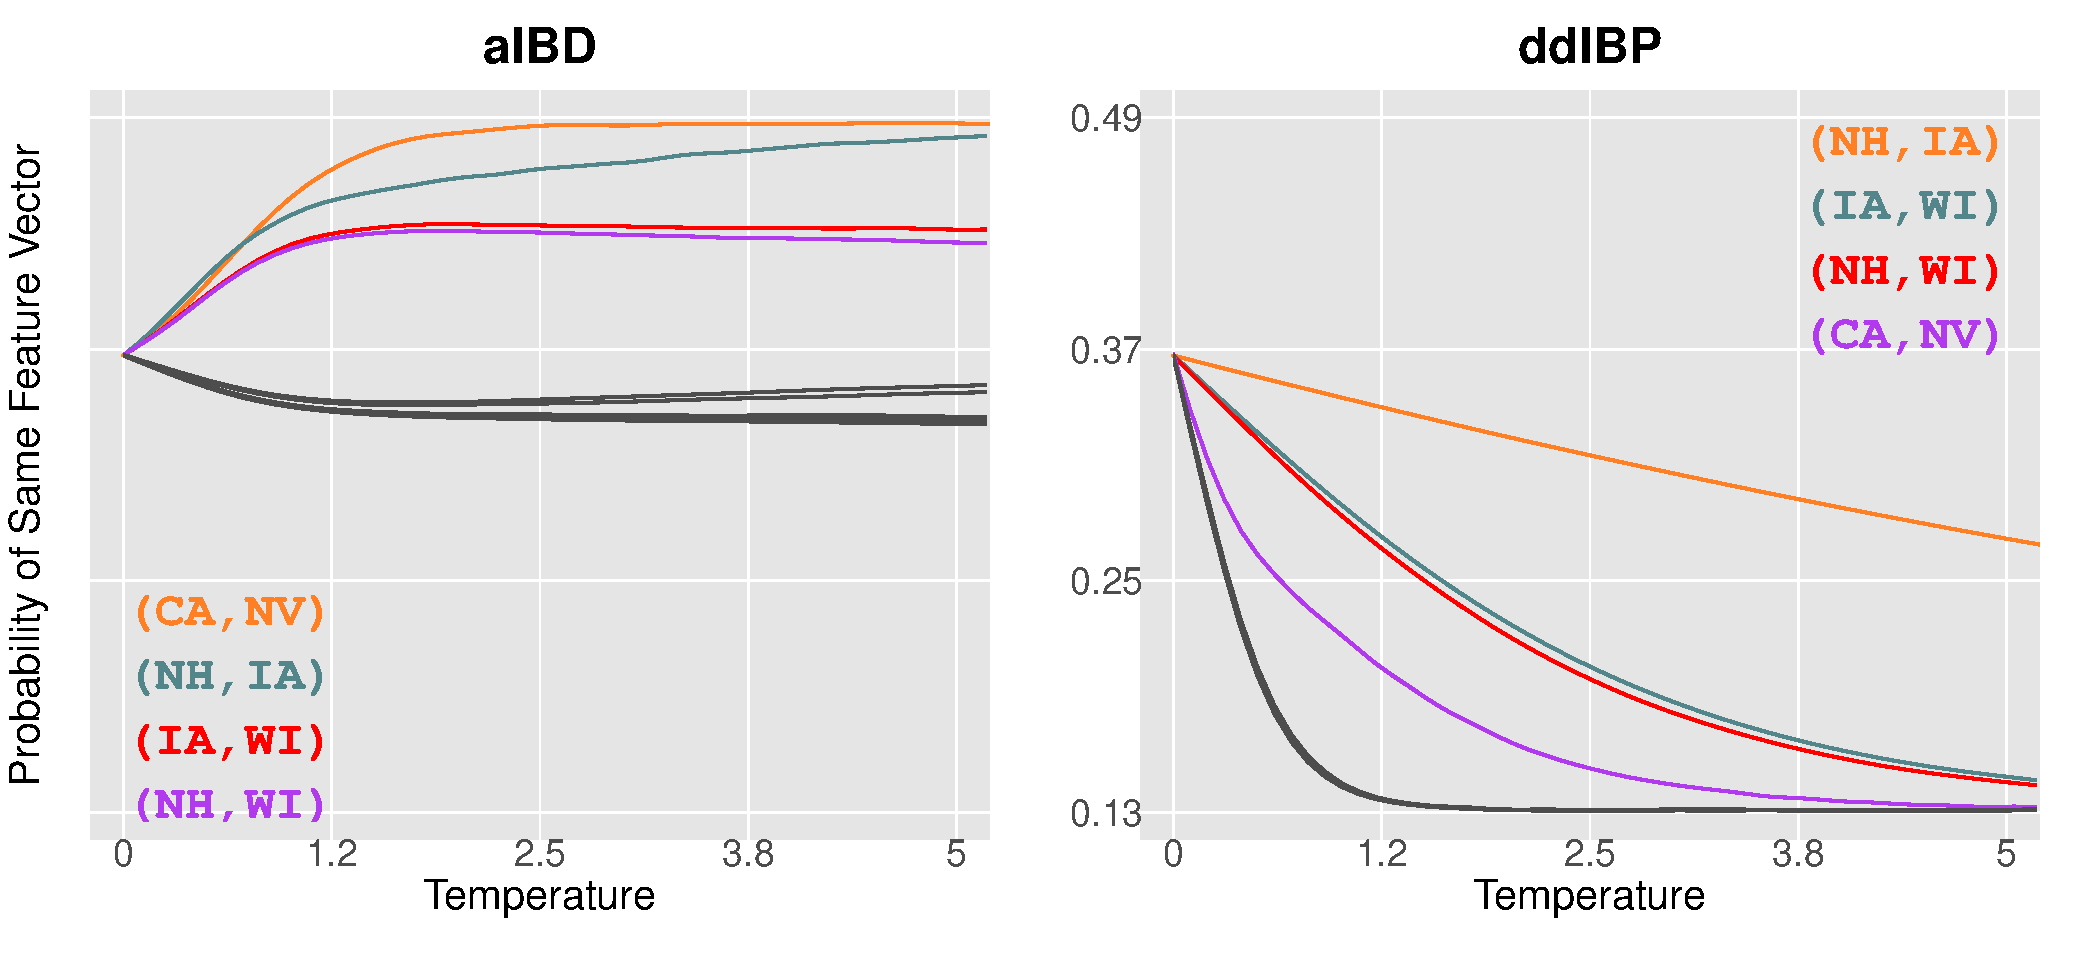
\includegraphics[width=.99\columnwidth,trim={0 0.7cm 0 0.3cm},clip]{temperatureArrest}}
          \\
          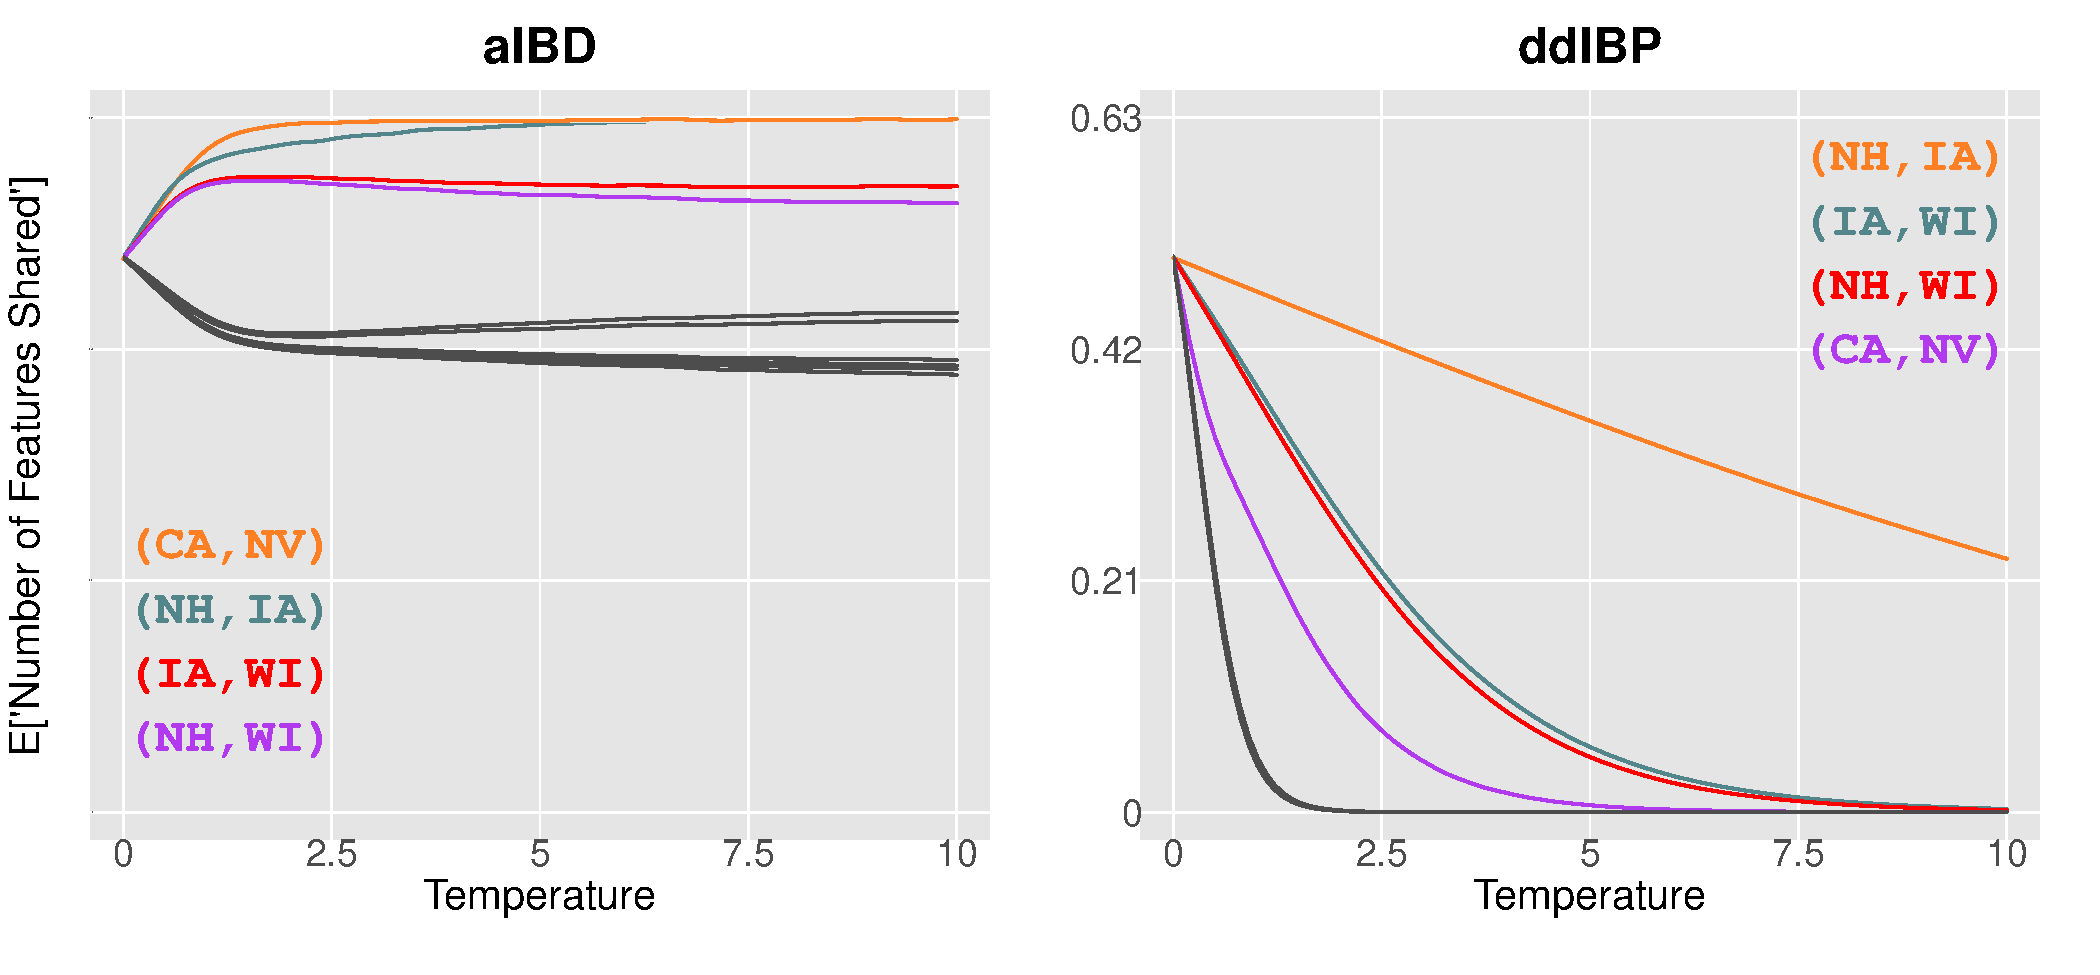
\includegraphics[width=.99\columnwidth,trim={0 0.7cm 0 0.3cm},clip]{sharedTemper}
        \end{figure}
      \end{block}

 
\vspace{1em}

       \begin{block}{Sampling Algorithm}
        To obtain a realization $\bm Z$ from an aIBD($\alpha$) with permutation
        \bm{$\sigma$} and distance $\bm D$: 
        \vspace{.5em}
        \begin{enumerate}
          \item The first customer $\sigma_1$ takes a Poisson($\alpha$) number of dishes.
          \item For customers $\sigma_i = 2\text{ to } N$,
          \begin{itemize}
            \item For each previously sampled dish,
              customer $\sigma_i$ takes dish $k$ with probability
              $h_{i,k}~m_{-i}/i$.
            \item After sampling all previously sampled dishes, customer
              $i$ samples Poisson($\alpha/i$) new dishes.
          \end{itemize}
        \end{enumerate}
      \end{block}






    \end{column}%1

    %-- Column 2 ---------------------------------------------------
    \begin{column}{0.56\linewidth}


     \begin{block}{Notation}
        Each row of the binary feature matrix $\bm Z$ denotes a ``customer''
        and each column represents a ``dish''. $z_{i,k}$ is set to 1 if
        customer $i$ takes dish $k$, and  0 otherwise. \\
        \vspace{1em}
        \begin{itemize}
          \setlength{\itemsep}{3pt}
          \item $x_i$ is the number of \textit{new} dishes that customer $i$ takes
            and $y_{i} = \suml{j}{1}{i-1} x_j$ is the number of existing dishes
            before customer $i$.
            %draws new dishes, for $i=\{2,...,N\}$. We will define $y_{-1} = 0$.
          \item $m_{-i,k}$ is the number of customers that took dish $k$ before customer
            customer $i$ samples dishes.
          %\item $m_{-i} = \suml{k}{1}{K}m_{-i,k}$ is the total number of dishes
            %taken before customer $i$ samples any dishes, where $K$ is the
            %number of non-zero columns in $\bm Z$.
          \item Let \\\hspace{.25\textwidth} $h_{i,k} = \hik$ \\
            be the similarity component of the weight
            given to sampling dish $k$ for customer $i$, where the permutation
            $\bm\sigma$ is the order in which customers are assigned dishes, 
            %Note that $\bm\sigma = (1,2,3,4,5)$ when the customers are
            %assigned in the order they appear in the dataset.
            and the similarity function $\lambda(i,j)$ maps the distance between
            customers $i$ and $j$ to a measure of how ``close'' the two customers
            are. 
            %$\lambda(i,j)$ can be rewritten as $f(d_{ij})$, where $f$ is some
            %non-increasing function such that $f(0)>0$ and $f(\infty)=0$, and
            %$d_{ij}$ is the distance between customers $i$ and $j$. 
            %Examples of $\lambda(i,j)=f(d_{ij})$ include: (i)
            %reciprocal similarity $f(d) = 1/d$, and (ii) exponential similarity
            %$f(d) = exp(-d)$.

          %\item The probability of customer $i$ drawing dish $k$ will be $p_{i,k} =
          %  h_{i,k} \ds\frac{m_{-i}}{i}$. Note that when $\lambda$ is a constant, $p_{i,k}$
          %  reduces to $m_{-i,k}$ as in the IBP.
        \end{itemize}
      \end{block}



      %  \vspace{1em}


      \begin{block}{Probability Mass Function}
        \[\Large
        \begin{array}{rrcl}
          \text{\textbf{IBP:\hspace{2.5em}}}
          &\text{P}(\bm Z|\alpha) & = & \frac{\alpha^{K}\exp\{-\alpha H_N\}}
                                     {\prodl{i}{1}{N}(i^{x_i}~x_i!)} 
                                \prodl{i}{2}{N}\prodl{k}{1}{y_{i}}
                                \left( \hspace{.39em}  \frac{m_{-i,k}}{i} \hspace{.39em}\right)^{z_{i,k}}
                                \left( \hspace{.30em}1-\frac{m_{-i,k}}{i} \hspace{.30em}\right)^{1-z_{i,k}}\\
          &&&\\
          %\text{\textbf{aIBD:~~~~~}}
          \text{\textbf{aIBD:\hspace{2.5em}}}
          &\text{P}(\bm{Z|D},\bm\sigma,\alpha) & = & 
                                \frac{\alpha^K \exp\{-\alpha H_N\}} 
                                     {\prodl{i}{1}{N}(i^{x_i}~x_i!)} 
                                \prodl{i}{2}{N}\prodl{k}{1}{y_i} 
                                \left( \frac{h_{i,k}   ~ (i-1)}{i} \right)^{z_{i,k}}
                                \left( 1-\frac{h_{i,k} ~ (i-1)}{i} \right)^{1-z_{i,k}}\\

        \end{array}  
        \]

        where $H_N = \suml{i}{1}{N} \ds\frac{1}{i}$ and $N$ is the total
        number of ``customers''.  \\ Note: If $y_i=0$ then the result of the product is 1.
      \end{block}

     %   \vspace{1em}

 \begin{block}{Demonstration}
        \hspace{4em}\textbf{US Arrest Dataset in R}
        \hspace{6em}\textbf{Euclidean Distance}
        \hspace{6.5em}\textbf{Similarity}
        \vspace{-.5em}
        \[
          %\input{figures/D.tex}
          \begin{tabular}{crrrrr}
\midrule   & Murder & Assault & Urban & Rape \\  \midrule
  NH & 2.1 & 57 & 56 & 9.5 \\ 
  IA & 2.2 & 56 & 57 & 11.3 \\ 
  WI & 2.6 & 53 & 66 & 10.8 \\ 
  CA & 9.0 & 276 & 91 & 40.6 \\ 
  NV & 12.2 & 252 & 81 & 46.0 \\ 
  \end{tabular} 

          \hspace{.5em}\rightarrow\hspace{.5em}
          \begin{tabular}{rrrrr}
\midrule  NH & IA & WI & CA & NV \\  \midrule
 0.00 & 0.12 & 0.66 & 3.74 & 3.78 \\ 
  0.12 & 0.00 & 0.59 & 3.65 & 3.69 \\ 
  0.66 & 0.59 & 0.00 & 3.32 & 3.46 \\ 
  3.74 & 3.65 & 3.32 & 0.00 & 1.01 \\ 
  3.78 & 3.69 & 3.46 & 1.01 & 0.00 \\ 
  \end{tabular} 

          \hspace{.5em}\rightarrow\hspace{.5em}
          %\input{figures/similarity.tex}
          \begin{tabular}{rrrrr}
\midrule  NH & IA & WI & CA & NV \\  \midrule
 1.00 & 0.89 & 0.51 & 0.02 & 0.02 \\ 
  0.89 & 1.00 & 0.55 & 0.03 & 0.02 \\ 
  0.51 & 0.55 & 1.00 & 0.04 & 0.03 \\ 
  0.02 & 0.03 & 0.04 & 1.00 & 0.36 \\ 
  0.02 & 0.02 & 0.03 & 0.36 & 1.00 \\ 
  \end{tabular} 

        \]

        \vspace{1em}
        \begin{figure}[htb]
          \centering
          \textbf{Expected Number of Shared Features}\\ \vspace{.5em}
          \raggedright{\small\textsf{\textbf{\hspace{8.5em}IBP \hspace{15.5em} aIBD \hspace{15em} ddIBP}}}\\
          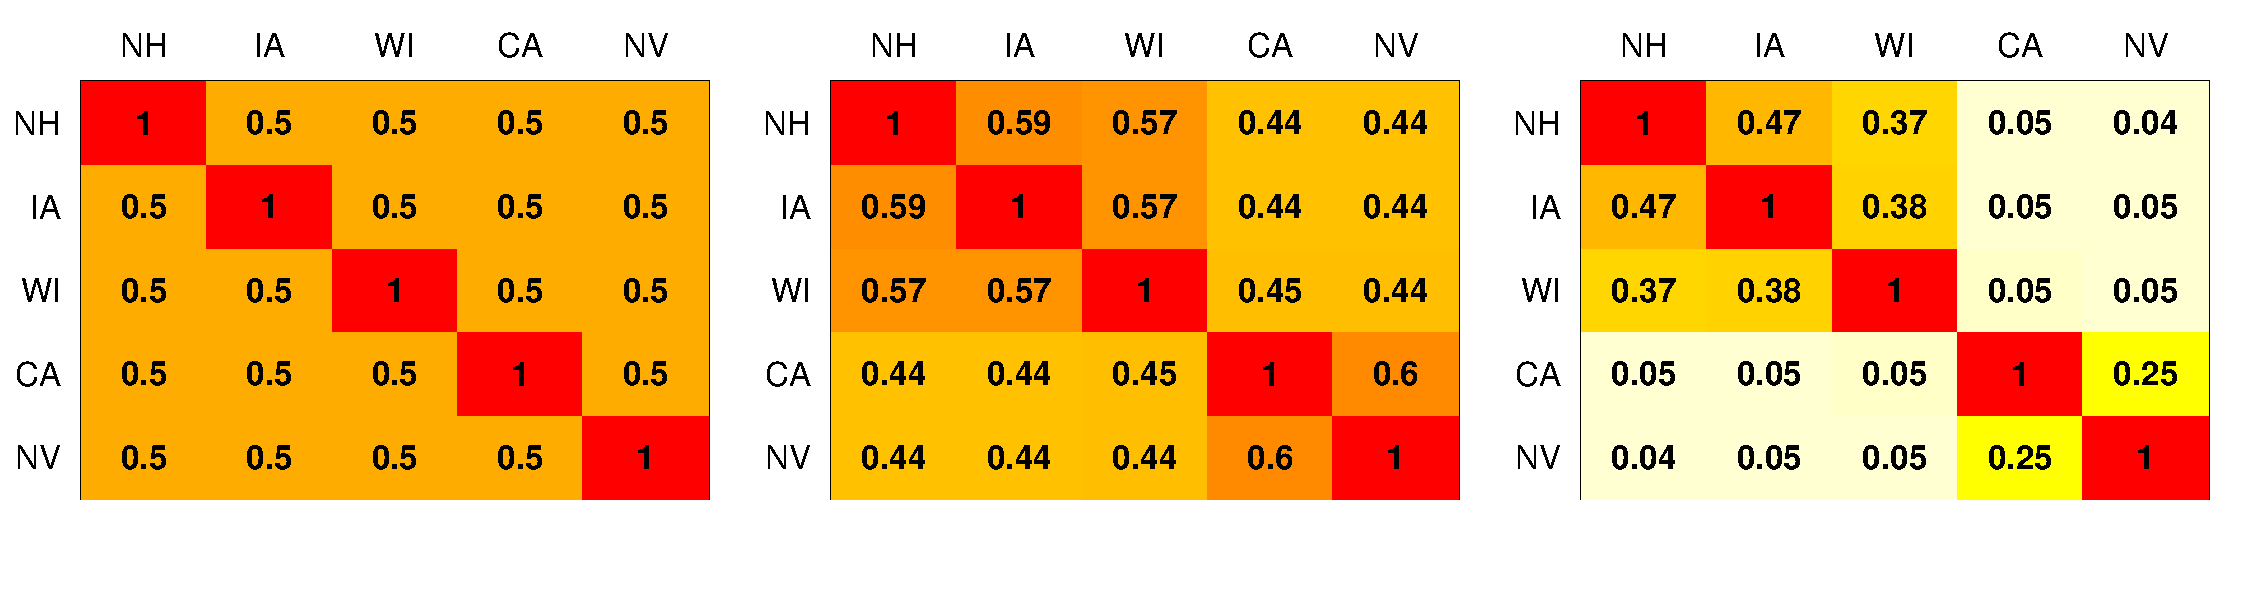
\includegraphics[width=.99\columnwidth]{sharedFeatures}
          %\includegraphics[width=.99\columnwidth]{heatPlots}

%          \centering
%        %\includegraphics[width=.99\columnwidth]{expect}
%          \textbf{Probability of Feature Given First Two Rows}\\ \vspace{.5em}
%          \raggedright{\small\textsf{\textbf{\hspace{8.5em}IBP \hspace{15.5em} aIBD \hspace{15em} ddIBP}}}\\
%          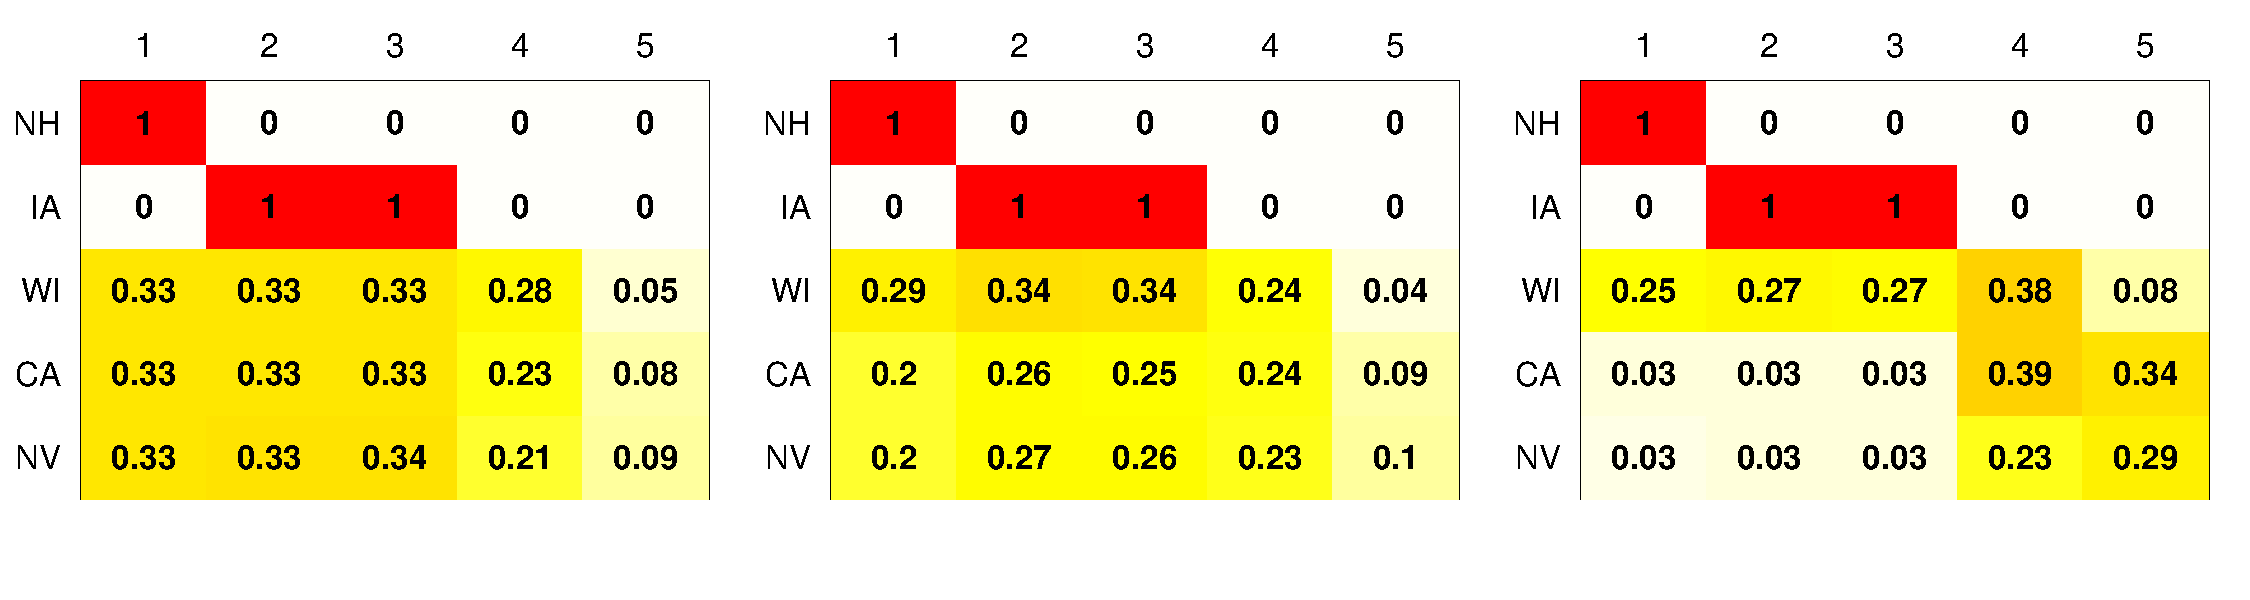
\includegraphics[width=.99\columnwidth]{expectArrest}\\
        \end{figure}
        \vspace{-2em}
      \end{block}










    \end{column}%2


  \end{columns}





      \begin{block}{References}
        \begin{itemize}
          \normalsize
          \item
            Blei, D. M. and Frazier, P.I. (2011),
            ``Distance Dependent Chinese Restaurant Process,"
            \emph{Journal of Machine Learning Research}, 12, 2383-2410.
          \item
            Dahl, D. B., Day, R., Tsai, J. W. (2017), ``Random Partition Distribution Indexed by Pairwise Information,"
              \emph{Journal of the American Statistical Association}, 112, 721-732.
          \item
            Gershman, S. J., Frazier, P.I., and Blei, D. M. (2015), ``Distance Dependent Infinite Latent Feature Models," \emph{IEEE Transactions on Pattern Analysis and Machine Intelligence}, 37, 334-345.
          \item
            Griffiths, T. L., and Ghahramani, Z. (2011), ``The Indian Buffet Process: An Introduction and Review," \emph{Journal of Machine Learning Research}, 12, 1185-1224.
          %\item
            %Neal, R. M. (2000), ``Markov Chain Sampling Methods for Dirichlet Process Mixture Models," \emph{Journal of Computational and Graphical Statistics}, 9, 249-265.
        \end{itemize}
      \end{block}




\end{frame}

\end{document}
